% Intro deck for the digital-twin workshop. Compile with: latexmk -xelatex intro.tex
\documentclass[aspectratio=169,11pt]{beamer}
\usetheme[progressbar=frametitle,numbering=fraction,block=fill]{metropolis}

\usepackage{tikz}
\usetikzlibrary{arrows.meta,positioning,shapes.geometric,shapes.symbols,calc,backgrounds,fit,decorations.pathmorphing}
\usepackage{pgfplots}
\pgfplotsset{compat=1.18}
\usepackage{fontawesome5}
\usepackage{booktabs}
\usepackage{ifthen}

% Colour code used in every drawing: orange = physical, teal = digital.
\definecolor{phys}{HTML}{E8743B}
\definecolor{digi}{HTML}{1B8A99}
\definecolor{ok}{HTML}{3C9A4E}
\definecolor{bad}{HTML}{C8323C}
\definecolor{ink}{HTML}{23373B}
\definecolor{soft}{HTML}{EEF1F2}
\definecolor{leaf}{HTML}{6FA35A}
\setbeamercolor{alerted text}{fg=phys}
\setbeamercolor{progress bar}{fg=digi,bg=soft}
\setbeamercolor{frametitle}{bg=ink}

\newcommand{\phys}[1]{\textcolor{phys}{\textbf{#1}}}
\newcommand{\digi}[1]{\textcolor{digi}{\textbf{#1}}}

\tikzset{
  box/.style={draw=#1, fill=#1!12, rounded corners=3pt, line width=0.9pt,
              minimum height=9mm, minimum width=22mm, align=center, font=\small},
  box/.default=ink,
  flow/.style={-{Stealth[length=2.6mm]}, line width=1pt, draw=ink!80},
  leafshape/.style={fill=leaf, draw=leaf!70!black, line width=0.4pt},
}
% A small potted plant: \plant{x}{y}{scale}
\newcommand{\plant}[3]{%
  \begin{scope}[shift={(#1,#2)}, scale=#3]
    \fill[phys!55!brown, draw=phys!40!black] (-0.35,0) -- (0.35,0) -- (0.45,0.5) -- (-0.45,0.5) -- cycle;
    \foreach \a/\r in {20/0.55, 60/0.7, 100/0.6, 140/0.75, 170/0.5, 80/0.85, 40/0.8}{
      \draw[leaf!60!black, line width=0.5pt] (0,0.5) -- ++(\a:\r*0.6);
      \fill[leafshape, rotate around={\a:($(0,0.5)+(\a:\r)$)}] ($(0,0.5)+(\a:\r)$) ellipse (0.28 and 0.14);
    }
  \end{scope}}

\title{A digital twin for a lab robot}
\subtitle{Test, acquire, simulate, evaluate --- before touching the machine}
\author{Aliénor Lahlou}
\date{Workshop · Jubilee digital twin}

\begin{document}

\begin{frame}[plain]
\begin{tikzpicture}[remember picture, overlay]
  \fill[ink] (current page.north west) rectangle ([yshift=-1.6cm]current page.north east);
  \node[anchor=north west, text=white, font=\Large\bfseries] at ([xshift=8mm, yshift=-4mm]current page.north west)
       {A digital twin for a lab robot};
  \node[anchor=north west, text=white!80, font=\small] at ([xshift=8mm, yshift=-10.5mm]current page.north west)
       {Test, acquire, simulate, evaluate --- before touching the machine};
  % physical photo and its twin, overlapping
  \node[inner sep=0, draw=phys, line width=2.5pt, rotate=-4] (r) at ([xshift=-3.9cm, yshift=-0.25cm]current page.center)
       {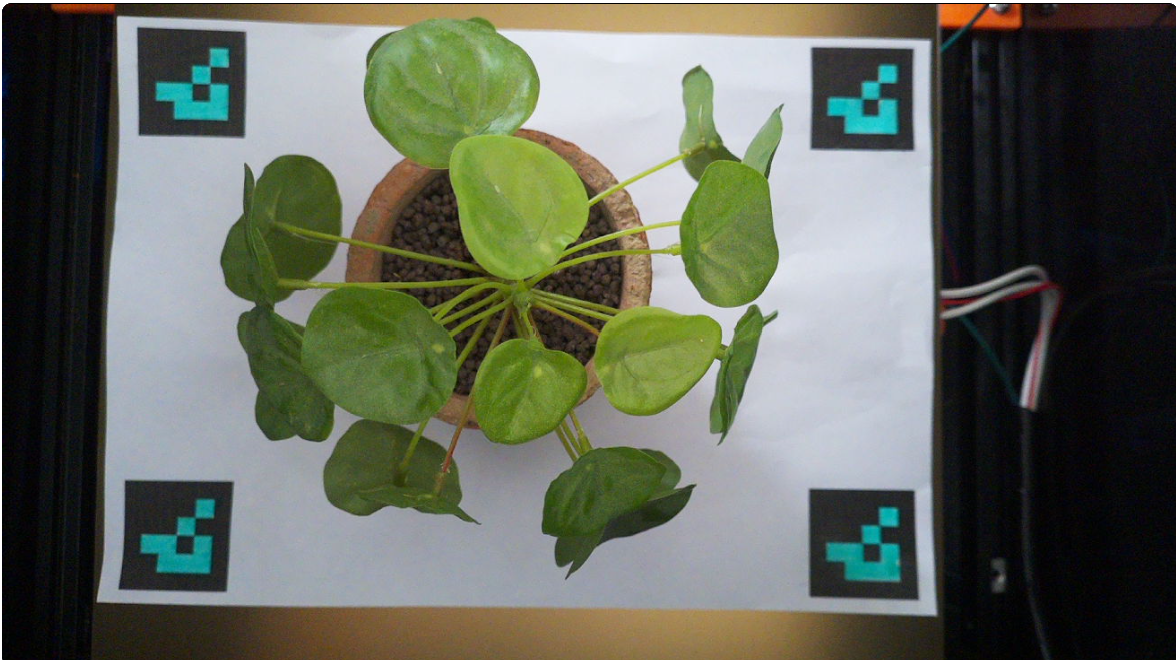
\includegraphics[width=6cm]{img/real_camera.png}};
  \node[inner sep=0, draw=digi, line width=2.5pt, rotate=3] (t) at ([xshift=3.0cm, yshift=-0.45cm]current page.center)
       {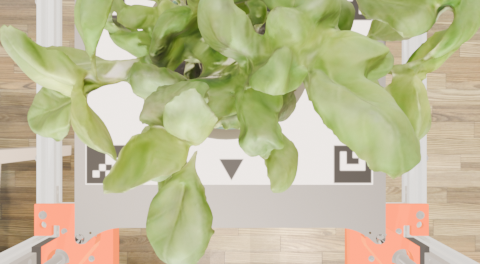
\includegraphics[width=6cm]{img/twin_camera.png}};
  \node[font=\small\bfseries, phys, below=2mm of r.south] {physical};
  \node[font=\small\bfseries, digi, below=2mm of t.south] {digital};
  \node[anchor=south west, font=\small, ink] at ([xshift=8mm, yshift=4mm]current page.south west)
       {Aliénor Lahlou · Jubilee digital-twin workshop};
\end{tikzpicture}
\end{frame}

% ─────────────────────────────────────────────────────────────────────────
\begin{frame}{Lab automation loves things that don't change}
\centering
\begin{tikzpicture}[x=1cm,y=1cm]
  % Left: a well plate, scripted once
  \begin{scope}
    \draw[rounded corners=4pt, line width=1pt, fill=soft] (0,0) rectangle (4.6,3);
    \foreach \i in {0,...,3} \foreach \j in {0,...,2}
      \draw[fill=white, draw=ink!60] (0.75+\i*1.03, 0.55+\j*0.95) circle (0.33);
    \draw[digi, line width=1.2pt, dashed, -{Stealth}] (0.75,0.55) -- (3.84,0.55) -- (3.84,1.5) -- (0.75,1.5) -- (0.75,2.45) -- (3.84,2.45);
    \node[font=\small\bfseries, ink] at (2.3,3.45) {Well plate};
    \node[font=\small, align=center, text width=6.4cm, anchor=north] at (2.3,-0.25)
      {Geometry known in advance\\[1pt]\textcolor{ok}{\faIcon{check}}\ \ write the path once, run it forever};
  \end{scope}
  % Right: a plant
  \begin{scope}[xshift=8cm]
    \draw[rounded corners=4pt, line width=1pt, fill=soft] (0,0) rectangle (4.6,3);
    \plant{2.3}{0.25}{1.45}
    \node[font=\Huge\bfseries, bad] at (4.15,2.55) {?};
    \node[font=\small\bfseries, ink] at (2.3,3.45) {Living sample};
    \node[font=\small, align=center, text width=6.4cm, anchor=north] at (2.3,-0.25)
      {Grows, moves, differs every time\\[1pt]\textcolor{bad}{\faIcon{times}}\ \ no path can be written in advance};
  \end{scope}
\end{tikzpicture}

\vspace{4mm}
\small Most self-driving labs require every object to be \emph{defined and hard-coded before the run}.
Plants, duckweed, tissues don't fit that paradigm.
\end{frame}

% ─────────────────────────────────────────────────────────────────────────
\begin{frame}{Vision fixes adaptability \dots\ and creates a safety problem}
\begin{columns}[c]
\column{0.5\textwidth}
\centering
\begin{tikzpicture}
  \node[box=digi, minimum width=24mm] (see) at (90:2) {\faIcon{camera}\\ see};
  \node[box=ink, minimum width=24mm] (dec) at (-30:2) {\faIcon{brain}\\ decide};
  \node[box=phys, minimum width=24mm] (mov) at (210:2) {\faIcon{route}\\ move};
  \draw[flow] (see) to[bend left=25] (dec);
  \draw[flow] (dec) to[bend left=25] (mov);
  \draw[flow] (mov) to[bend left=25] (see);
  \node[starburst, starburst points=9, fill=bad, draw=bad!70!black, text=white,
        font=\scriptsize\bfseries, minimum size=16mm, align=center] at (215:3.9) {crash};
\end{tikzpicture}
\column{0.48\textwidth}
\textbf{(A) Adaptability.} The robot looks at the sample and decides where to go.

\vspace{3mm}
\textbf{(B) Safety.} A robot that decides its own moves can also decide to hit
the sample, the labware, or itself --- moves nobody reviewed.

\vspace{3mm}
\alert{That's why vision-driven robots are usually kept away from living samples.}
\end{columns}
\end{frame}

% ─────────────────────────────────────────────────────────────────────────
\begin{frame}{The idea: every move goes through the twin first}
\centering
\begin{tikzpicture}[node distance=7mm]
  \node[box=phys] (scan) {\faIcon{camera}\\ Scan};
  \node[box=ink, right=of scan] (target) {\faIcon{crosshairs}\\ Target};
  \node[box=digi, right=of target, minimum width=30mm, minimum height=14mm, line width=1.6pt] (val)
       {\faIcon{cube}\ \textbf{Validate}\\ \footnotesize in the digital twin};
  \node[box=phys, right=14mm of val] (act) {\faIcon{robot}\\ Act};
  \draw[flow] (scan) -- (target);
  \draw[flow] (target) -- (val);
  \draw[flow, draw=ok] (val) -- node[above, font=\scriptsize, ok]{safe} (act);
  \draw[flow, draw=bad] (val.south) -- ++(0,-0.75) -| node[pos=0.25, below, font=\scriptsize, bad]{collision: re-plan} (target.south);
  \draw[flow, draw=ink!40, dashed] (act.north) -- ++(0,0.8) -| node[pos=0.25, above, font=\scriptsize, ink!70]{observe the result} (scan.north);
  % Physical / digital bands
  \begin{scope}[on background layer]
    \node[fill=digi!7, rounded corners=6pt, fit=(val), inner sep=5mm] {};
  \end{scope}
\end{tikzpicture}

\vspace{6mm}
\begin{columns}[t]
\column{0.3\textwidth}\centering \phys{Physical}\\ \footnotesize the real Jubilee and its camera
\column{0.3\textwidth}\centering \digi{Digital}\\ \footnotesize a synchronized 3D copy in Blender
\column{0.3\textwidth}\centering \textbf{Rule}\\ \footnotesize nothing reaches the motors without passing the twin
\end{columns}
\end{frame}

% ─────────────────────────────────────────────────────────────────────────
\begin{frame}{Model, shadow, twin: it's about which way the data flows}
\centering
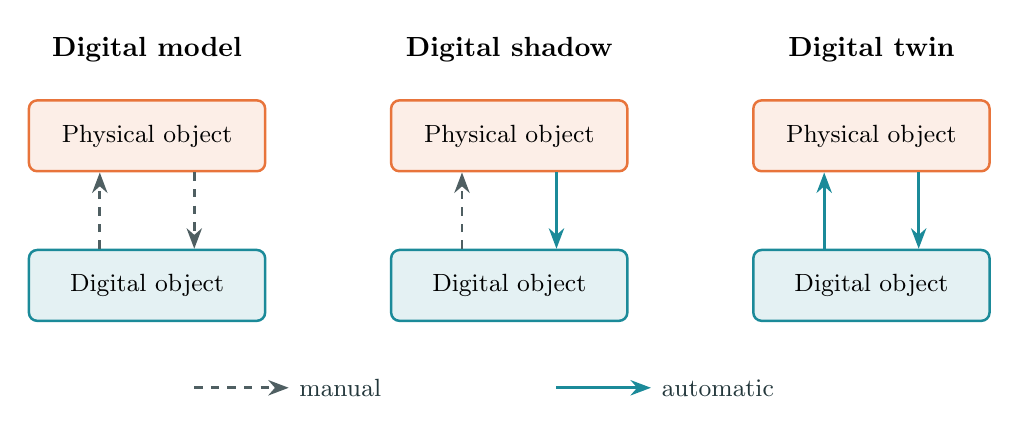
\begin{tikzpicture}[x=1cm,y=1cm]
  \foreach \x/\name/\up/\down in {0/Digital model/manual/manual, 4.6/Digital shadow/manual/auto, 9.2/Digital twin/auto/auto}{
    \begin{scope}[xshift=\x cm]
      \node[font=\bfseries] at (1.6,3.3) {\name};
      \node[box=phys, minimum width=30mm] (P) at (1.6,2.2) {Physical object};
      \node[box=digi, minimum width=30mm] (D) at (1.6,0.3) {Digital object};
      \ifthenelse{\equal{\down}{auto}}
        {\draw[flow, draw=digi] ([xshift=6mm]P.south) -- ([xshift=6mm]D.north);}
        {\draw[flow, dashed] ([xshift=6mm]P.south) -- ([xshift=6mm]D.north);}
      \ifthenelse{\equal{\up}{auto}}
        {\draw[flow, draw=digi] ([xshift=-6mm]D.north) -- ([xshift=-6mm]P.south);}
        {\draw[flow, dashed] ([xshift=-6mm]D.north) -- ([xshift=-6mm]P.south);}
    \end{scope}}
  \draw[flow, dashed] (2.2,-1) -- ++(1.2,0) node[right, font=\small, ink]{manual};
  \draw[flow, draw=digi] (6.8,-1) -- ++(1.2,0) node[right, font=\small, ink]{automatic};
\end{tikzpicture}

\vspace{2mm}
\small A twin is \emph{kept in sync} with the machine (positions, tools, calibration)
and \emph{talks back} to it (which moves are allowed).
\end{frame}

% ─────────────────────────────────────────────────────────────────────────
\begin{frame}{The machine: Jubilee, with a camera on the toolhead}
\begin{columns}[c]
\column{0.56\textwidth}
\centering
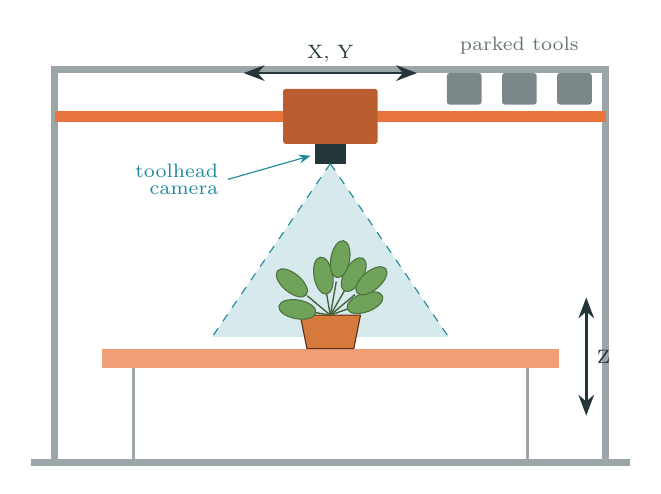
\begin{tikzpicture}[x=1cm,y=1cm]
  % frame
  \draw[line width=2.5pt, ink!45] (0,0) -- (0,5) -- (7,5) -- (7,0);
  \draw[line width=2.5pt, ink!45] (-0.3,0) -- (7.3,0);
  % gantry + carriage + camera
  \draw[line width=4pt, phys] (0,4.4) -- (7,4.4);
  \fill[phys!80!black, rounded corners=1pt] (2.9,4.05) rectangle (4.1,4.75);
  \fill[ink] (3.3,3.8) rectangle (3.7,4.05);
  \fill[digi, opacity=0.18] (3.5,3.8) -- (2.0,1.6) -- (5.0,1.6) -- cycle;
  \draw[digi, dashed] (3.5,3.8) -- (2.0,1.6) (3.5,3.8) -- (5.0,1.6);
  % parked tools
  \foreach \x in {5.2,5.9,6.6} \fill[ink!60, rounded corners=1pt] (\x-0.22,4.55) rectangle (\x+0.22,4.95);
  \node[font=\scriptsize, ink!70] at (5.9,5.3) {parked tools};
  % bed + plant
  \fill[phys!70] (0.6,1.2) rectangle (6.4,1.45);
  \draw[ink!45, line width=1.2pt] (1,1.2) -- (1,0) (6,1.2) -- (6,0);
  \plant{3.5}{1.45}{0.85}
  % axis annotations
  \draw[{Stealth}-{Stealth}, line width=1pt, ink] (2.4,4.95) -- (4.6,4.95) node[midway, above, font=\scriptsize]{X, Y};
  \draw[{Stealth}-{Stealth}, line width=1pt, ink] (6.75,0.6) -- (6.75,2.1) node[midway, right, font=\scriptsize]{Z};
  \node[font=\scriptsize, digi, align=right, anchor=east] (camlbl) at (2.2,3.6) {toolhead\\[-2pt]camera};
  \draw[digi, -{Stealth[length=1.5mm]}] (camlbl.east) -- (3.25,3.9);
\end{tikzpicture}
\column{0.42\textwidth}
\small
\begin{itemize}
  \item Open-source \textbf{tool-changing} motion platform
  \item \textbf{X/Y} move the toolhead (and the camera)
  \item \textbf{Z} moves the \emph{bed}: bigger Z $=$ bed lower $=$ sample further from the camera
  \item Tools: camera, inoculator, pen, fluorescence probe\dots
\end{itemize}
\vspace{2mm}
\footnotesize You'll need the Z convention in Exercise 1.
\end{columns}
\end{frame}

% ─────────────────────────────────────────────────────────────────────────
\begin{frame}{One machine, two copies}
\centering
\begin{tikzpicture}
  \node[inner sep=0, draw=phys, line width=2pt] (real) at (0,0) {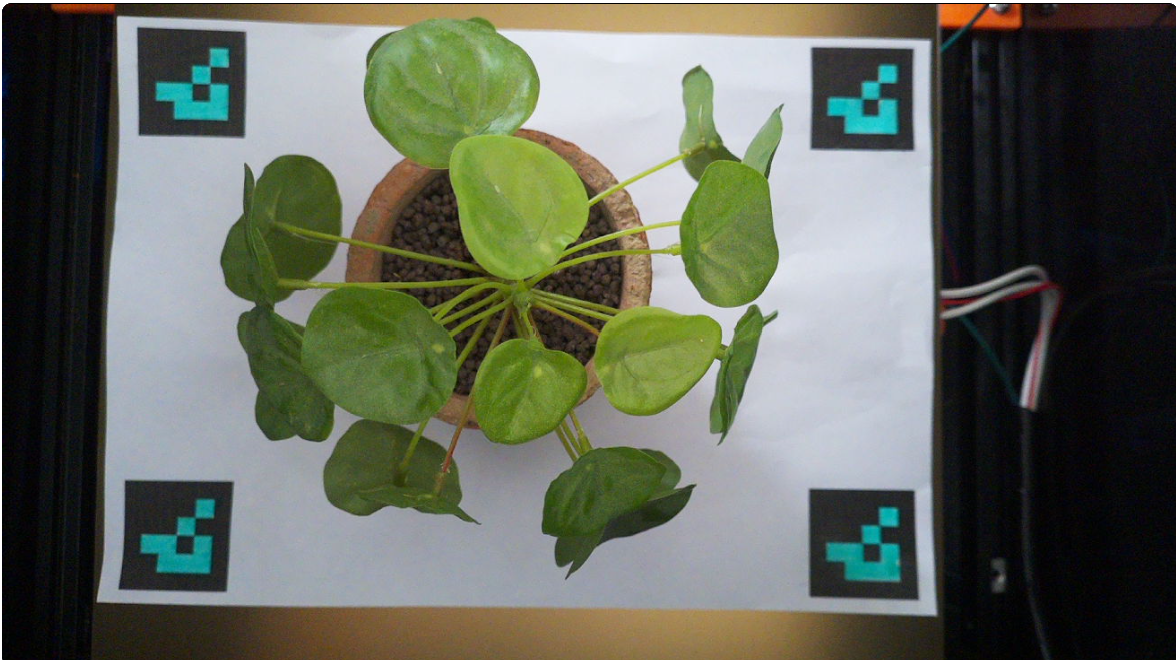
\includegraphics[height=3.1cm]{img/real_camera.png}};
  \node[inner sep=0, draw=digi, line width=2pt, right=22mm of real] (twin) {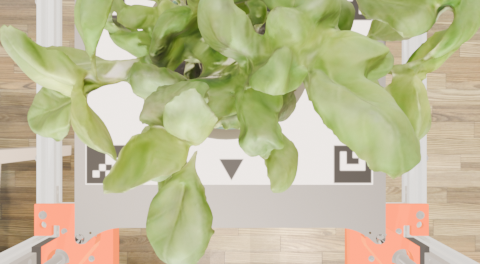
\includegraphics[height=3.1cm]{img/twin_camera.png}};
  \node[above=1mm of real, font=\small\bfseries, phys] {real toolhead camera};
  \node[above=1mm of twin, font=\small\bfseries, digi] {\texttt{Toolhead\_Cam} in Blender};
  \draw[flow, line width=1.4pt] (real.east) -- node[above, font=\scriptsize, align=center]{same\\calibration} (twin.west);
\end{tikzpicture}

\vspace{4mm}
\begin{columns}[t]
\column{0.47\textwidth}\footnotesize
\textbf{Geometry from the machine}: tool slots, park positions, offsets and head position are read
from the Duet (or a saved snapshot), so the scene matches the real deck.
\column{0.47\textwidth}\footnotesize
\textbf{Camera from calibration}: the pinhole intrinsics $f_x, f_y, c_x, c_y$ become Blender's lens and shift,
so a pixel in the twin means the same thing as a pixel on the machine.
\end{columns}
\end{frame}

% ─────────────────────────────────────────────────────────────────────────
\begin{frame}{How the twin is wired}
\centering
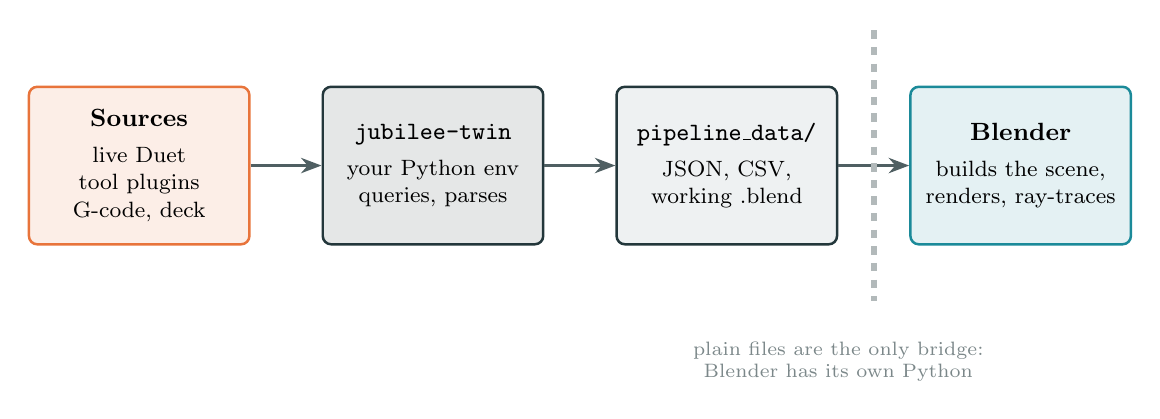
\begin{tikzpicture}[node distance=9mm]
  \node[box=phys, minimum width=28mm, minimum height=20mm] (src)
    {\textbf{Sources}\\[2pt]\footnotesize live Duet\\[-1pt]\footnotesize tool plugins\\[-1pt]\footnotesize G-code, deck};
  \node[box=ink, right=of src, minimum width=28mm, minimum height=20mm] (cli)
    {\texttt{jubilee-twin}\\[2pt]\footnotesize your Python env\\[-1pt]\footnotesize queries, parses};
  \node[box=ink, right=of cli, minimum width=28mm, minimum height=20mm, fill=soft] (pd)
    {\texttt{pipeline\_data/}\\[2pt]\footnotesize JSON, CSV,\\[-1pt]\footnotesize working .blend};
  \node[box=digi, right=of pd, minimum width=28mm, minimum height=20mm] (bl)
    {\textbf{Blender}\\[2pt]\footnotesize builds the scene,\\[-1pt]\footnotesize renders, ray-traces};
  \draw[flow] (src) -- (cli); \draw[flow] (cli) -- (pd); \draw[flow] (pd) -- (bl);
  \draw[line width=2pt, ink!35, dashed] ($(pd.north east)!0.5!(bl.north west)+(0,0.7)$) -- ($(pd.south east)!0.5!(bl.south west)+(0,-0.7)$);
  \node[font=\scriptsize, ink!60, align=center, below=11mm of pd.south east, anchor=north] {plain files are the only bridge:\\Blender has its own Python};
\end{tikzpicture}

\vspace{2mm}
\small Every number in the scene comes from a file you can open --- and a trace page says which source won.
\end{frame}

% ─────────────────────────────────────────────────────────────────────────
\begin{frame}{The collision gate: rays along the motion}
\begin{columns}[c]
\column{0.52\textwidth}
\centering
\begin{tikzpicture}[x=1cm,y=1cm]
  % gantry hull
  \fill[digi!15, draw=digi, line width=1pt] (0,1.2) -- (0.4,2.4) -- (1.6,2.6) -- (2.2,1.8) -- (1.8,0.8) -- (0.6,0.6) -- cycle;
  \node[font=\scriptsize, digi] at (1.1,1.65) {gantry hull};
  % motion
  \draw[-{Stealth[length=3mm]}, line width=2pt, phys] (0.4,3.1) -- (2.4,3.1) node[right, font=\scriptsize]{next move};
  % plant leaves in the way
  \fill[leafshape, rotate around={15:(4.45,1.85)}] (4.45,1.85) ellipse (0.6 and 0.26);
  \fill[leafshape, rotate around={-10:(4.35,0.8)}] (4.35,0.8) ellipse (0.55 and 0.24);
  % rays from hull vertices: two end on a leaf, the others pass
  \foreach \p in {(0.4,2.4),(1.6,2.6),(0.6,0.6),(0,1.2)}
    \draw[-{Stealth[length=1.6mm]}, ink!70] \p -- ++(2.6,0);
  \draw[bad, line width=1pt] (2.2,1.8) -- (3.88,1.8);
  \draw[bad, line width=1pt] (1.8,0.8) -- (3.82,0.8);
  \foreach \p in {(3.88,1.8),(3.82,0.8)}
    \node[bad, font=\large\bfseries] at \p {\faIcon{times}};
  \node[font=\scriptsize, bad, align=center] at (4.4,-0.1) {hit $\Rightarrow$ collision\\at this frame};
\end{tikzpicture}
\column{0.46\textwidth}
\footnotesize
For each frame of the planned motion:
\begin{enumerate}
  \item take the convex hull of the moving parts (+ active tool)
  \item cast rays from its vertices, along the motion
  \item any scene object hit $=$ collision, with frame and object name
\end{enumerate}
\vspace{1mm}
\centering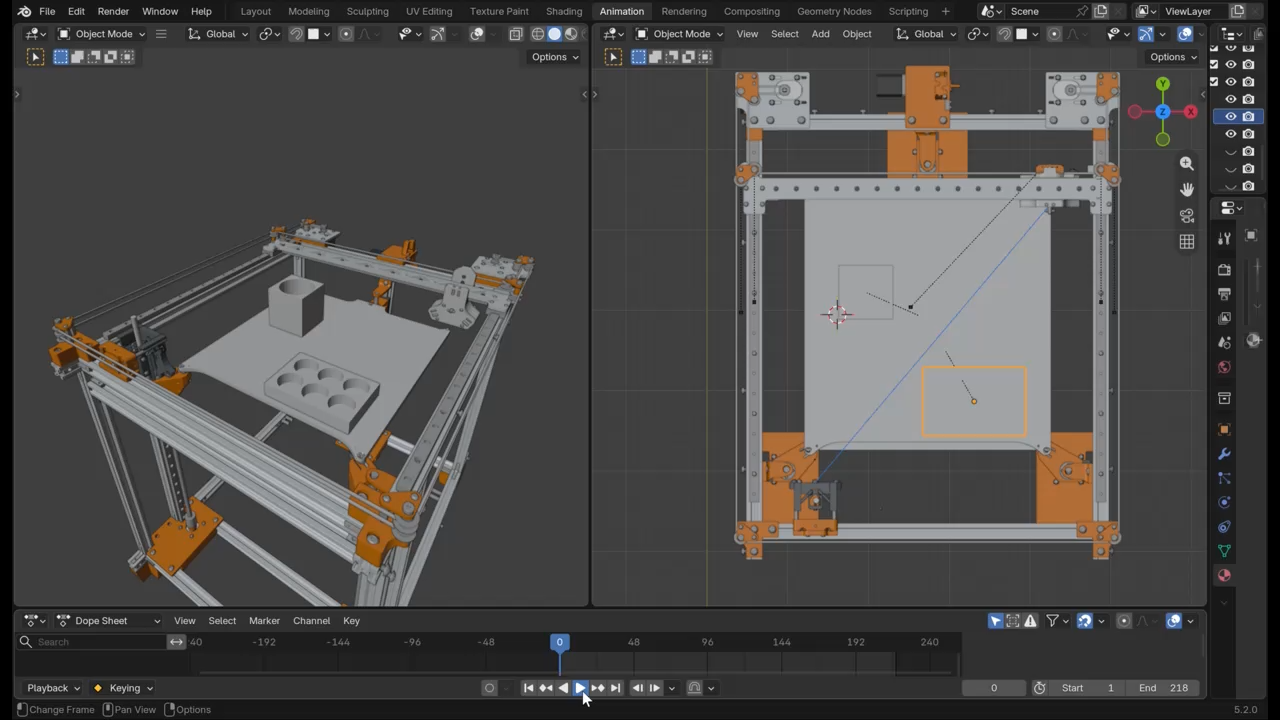
\includegraphics[width=0.62\linewidth]{img/raycast_viewport.png}
\end{columns}
\end{frame}

% ─────────────────────────────────────────────────────────────────────────
\begin{frame}{What a twin unlocks}
\centering
\begin{tikzpicture}[x=1cm,y=1cm]
  \foreach \i/\x/\y/\icon/\ttl/\txt in {
      1/0/2.6/\faIcon{shield-alt}/{Test before running}/{Find the crash in the twin\\ instead of on the machine},
      2/7.2/2.6/\faIcon{camera}/{Acquire virtually}/{Script and debug an acquisition\\ that makes its own decisions},
      3/0/0/\faIcon{images}/{Synthetic data}/{Unlimited images with labels\\ (depth, masks, poses) for free},
      4/7.2/0/\faIcon{ruler-combined}/{An exact yardstick}/{Score 3D vision models against\\ geometry we know exactly}}{
    \node[box=digi, minimum width=62mm, minimum height=21mm, anchor=south west, align=left, fill=digi!6] at (\x,\y) {};
    \node[anchor=west, font=\LARGE, digi] at (\x+0.35,\y+1.05) {\icon};
    \node[anchor=north west, font=\small\bfseries, ink] at (\x+1.35,\y+1.85) {\ttl};
    \node[anchor=north west, font=\footnotesize, ink, align=left] at (\x+1.35,\y+1.3) {\txt};
    \node[anchor=north east, font=\scriptsize\bfseries, phys] at (\x+6.1,\y+2) {Ex.\,\i};
  }
\end{tikzpicture}
\end{frame}

% ─────────────────────────────────────────────────────────────────────────
\begin{frame}{\faIcon{shield-alt}\ \ Unlock 1 --- test before running}
\begin{columns}[c]
\column{0.5\textwidth}

\includegraphics[width=\linewidth]{img/crash_view.png}
\par\centering\footnotesize What the toolhead camera sees\\ a moment before a crash.
\column{0.46\textwidth}
\small
An old plan, written for a flat Petri dish. Today there's a basil plant on the bed.

\vspace{3mm}
In the twin you can:
\begin{itemize}
  \item replay the G-code and get every colliding frame
  \item ask questions you'd never ask the real machine: \emph{what's the lowest Z that's still safe?}
\end{itemize}
\vspace{2mm}
\alert{A crash in the twin costs about 15 seconds.}
\end{columns}
\end{frame}

% ─────────────────────────────────────────────────────────────────────────
\begin{frame}{\faIcon{camera}\ \ Unlock 2 --- acquisitions that decide}
\centering
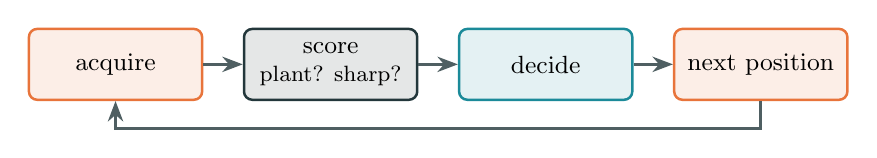
\begin{tikzpicture}[node distance=5mm]
  \node[box=phys] (acq) {acquire};
  \node[box=ink, right=of acq] (score) {score\\[-1pt]\footnotesize plant? sharp?};
  \node[box=digi, right=of score] (dec) {decide};
  \node[box=phys, right=of dec] (next) {next position};
  \draw[flow] (acq) -- (score); \draw[flow] (score) -- (dec); \draw[flow] (dec) -- (next);
  \draw[flow] (next.south) -- ++(0,-0.35) -| (acq.south);
\end{tikzpicture}

\vspace{3mm}
\begin{columns}[c]
\column{0.62\textwidth}
\centering
\begin{tikzpicture}
  \foreach \img/\lbl [count=\k] in {focus_worst/bed too high, focus_mid/closer, focus_best/in focus}
    \node[inner sep=0, label={[font=\scriptsize]below:\lbl}] at (\k*3.05,0) {\includegraphics[width=2.9cm]{img/\img.png}};
\end{tikzpicture}
\column{0.36\textwidth}
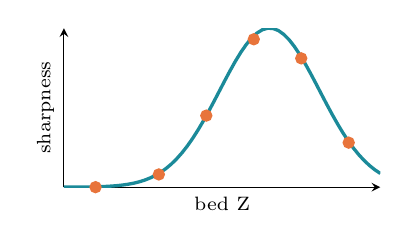
\begin{tikzpicture}
  \begin{axis}[width=5.6cm, height=3.6cm, xlabel={\scriptsize bed Z}, ylabel={\scriptsize sharpness},
               ticks=none, axis lines=left, every axis plot/.append style={line width=1.2pt}]
    \addplot[digi, domain=0:10, samples=60] {exp(-(x-6.5)^2/5)+0.05};
    \addplot[only marks, mark=*, phys, mark size=1.6pt] coordinates {(1,0.05)(3,0.13)(4.5,0.5)(6,0.98)(7.5,0.86)(9,0.33)};
  \end{axis}
\end{tikzpicture}
\end{columns}

\vspace{1mm}
\small The virtual camera has a real depth of field, so autofocus is a genuine decision.
\end{frame}

% ─────────────────────────────────────────────────────────────────────────
\begin{frame}{\faIcon{images}\ \ Unlock 3 --- same geometry, many appearances}
\centering
\begin{tikzpicture}
  \foreach \img/\lbl [count=\k] in {look_kitchen/kitchen HDRI, look_forest/forest HDRI, look_studio/studio HDRI, look_plain/plain background}
    \node[inner sep=0, label={[font=\scriptsize]above:\lbl}] at (\k*3.25,0) {\includegraphics[width=3.1cm]{img/\img.png}};
  \draw[decorate, decoration={brace, amplitude=6pt, mirror}, line width=1pt, ink]
       (1.7,-0.95) -- (14.55,-0.95);
  \node[font=\footnotesize\bfseries, ink] at (8.12,-1.4) {identical labels for every look};
  \node[inner sep=0, label={[font=\scriptsize]below:depth}] (d) at (4.9,-2.75) {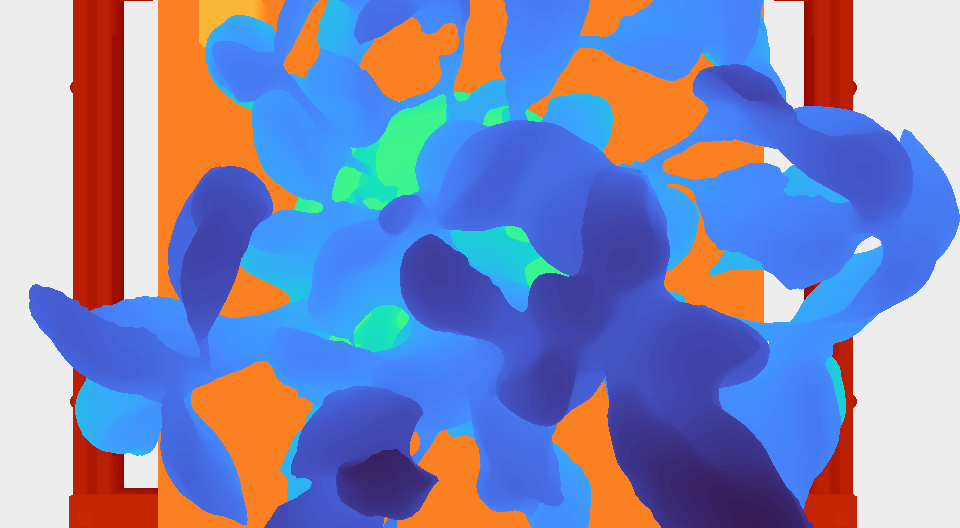
\includegraphics[width=3.1cm]{img/gt_depth.png}};
  \node[inner sep=0, label={[font=\scriptsize]below:plant mask}] (m) at (8.15,-2.75) {
\includegraphics[width=3.1cm]{img/gt_mask.png}};
  \node[box=digi, right=5mm of m, minimum width=26mm, font=\footnotesize] {$K$, camera pose,\\full 3D mesh};
\end{tikzpicture}

\vspace{1mm}
\small An \textbf{HDRI} is a 360° photo that both lights the scene and is the background.
Swap it and the appearance changes, but the annotations don't.
\end{frame}

% ─────────────────────────────────────────────────────────────────────────
\begin{frame}{\faIcon{ruler-combined}\ \ Unlock 4 --- a yardstick for 3D vision}
\begin{columns}[c]
\column{0.42\textwidth}
\centering
\phys{Real plant}\\[1mm]
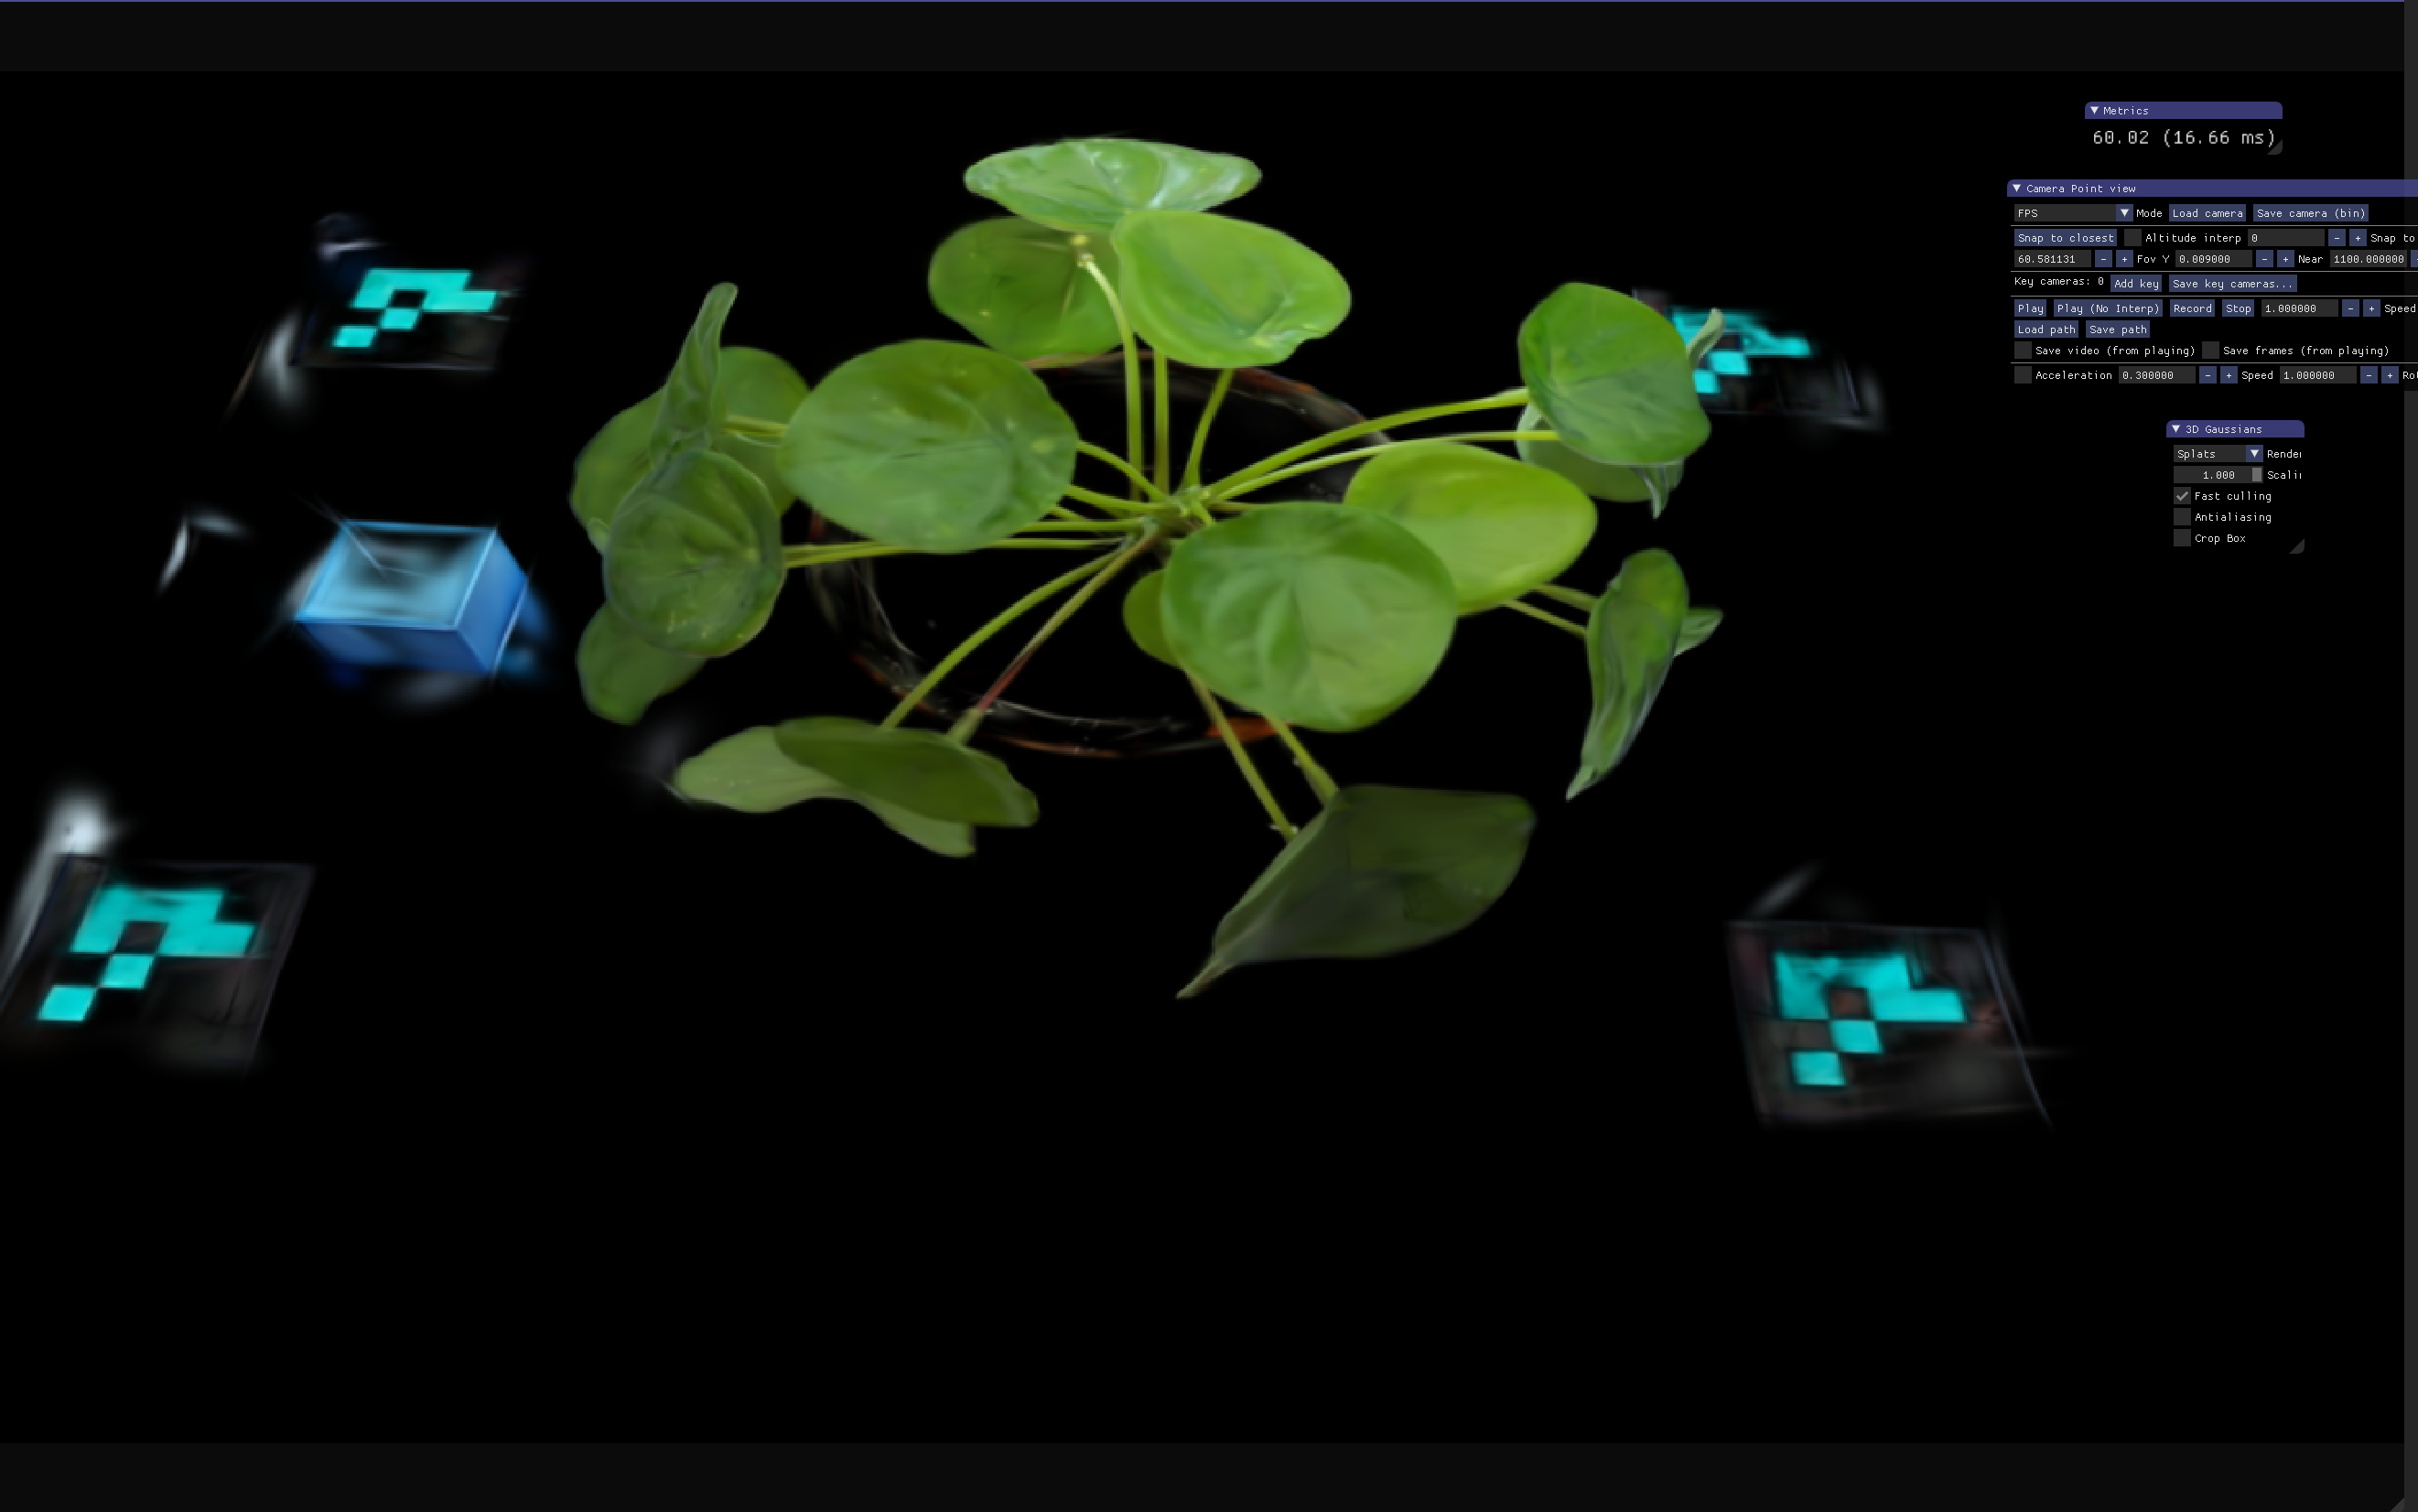
\includegraphics[width=0.82\linewidth]{img/gs_reconstruction.png}\\[1mm]
\footnotesize Gaussian-splatting reconstruction. It looks right, but \emph{how} right?\\
No ground truth exists.
\column{0.56\textwidth}
\centering
\digi{Twin plant}\\[1mm]
\begin{tikzpicture}[x=1cm, y=1cm]
  \node[inner sep=0, draw=digi, line width=1.2pt] (img) at (0,0) {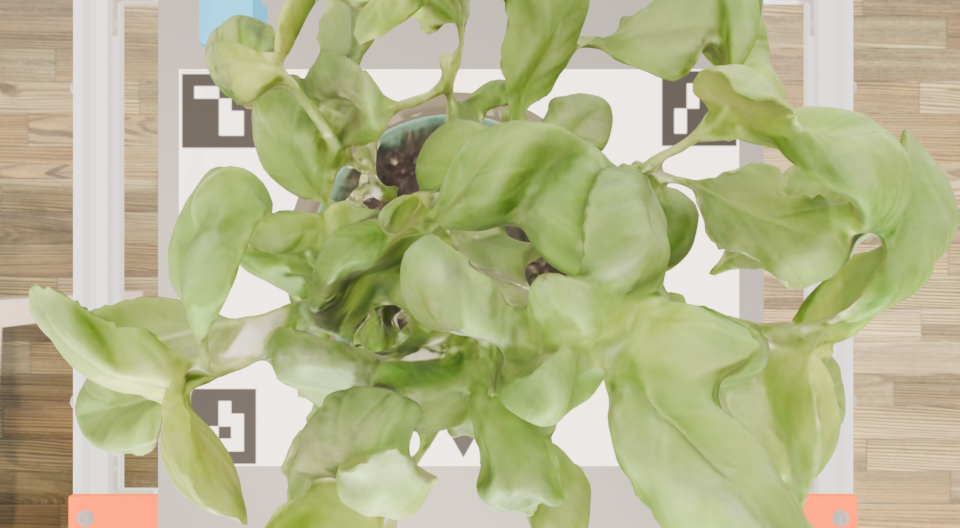
\includegraphics[width=2.7cm]{img/moge_input.png}};
  \node[box=ink, minimum width=19mm, minimum height=8mm, font=\footnotesize] (m) at (3.2,0.55) {MoGe-2\\[-2pt]\scriptsize one image};
  \node[box=digi, minimum width=19mm, minimum height=8mm, font=\footnotesize] (rc) at (3.2,-0.55) {ray casting\\[-2pt]\scriptsize exact};
  \draw[flow] (img.east) ++(0,0.3) -- (m.west);
  \draw[flow] (img.east) ++(0,-0.3) -- (rc.west);
  % nearest-neighbour illustration: predicted points (orange) vs true surface (green)
  \begin{scope}[shift={(-1.3,-2.75)}, x=0.95cm, y=0.95cm]
    \draw[ok!60, line width=1.5pt, domain=0:5.2, samples=60, smooth] plot (\x, {0.45*sin(\x*70)});
    \foreach \t in {0,0.5,...,5}{
      \pgfmathsetmacro{\yg}{0.45*sin(\t*70)}
      \pgfmathsetmacro{\yp}{0.55*sin(\t*70)+0.32}
      \draw[ink!50] (\t+0.1,\yp) -- (\t,\yg);
      \fill[phys] (\t+0.1,\yp) circle (2.4pt);
    }
    \node[anchor=west, font=\scriptsize, phys] at (5.35,0.55) {prediction};
    \node[anchor=west, font=\scriptsize, ok!70!black] at (5.35,-0.05) {true surface};
    \node[anchor=west, font=\scriptsize, ink!70] at (5.35,-0.6) {nearest distance};
  \end{scope}
  \draw[flow, ink!50] (m.south east) ++(0.2,0) to[out=-60, in=60] (4.0,-1.75);
\end{tikzpicture}
\end{columns}

\vspace{2mm}
\small Same camera, same image, so the clouds are directly comparable. Distances to the true surface
give \textbf{scale error}, \textbf{accuracy}, \textbf{completeness} and \textbf{Chamfer distance}.
\end{frame}

% ─────────────────────────────────────────────────────────────────────────
\begin{frame}{Where this is going: closing the loop}
\centering
\begin{tikzpicture}
  \def\R{2.25}
  \node[box=phys, minimum width=30mm] (mach) at (90:\R) {\faIcon{robot}\ machine};
  \node[box=phys, minimum width=30mm] (img)  at (0:\R*1.55) {\faIcon{camera}\ images};
  \node[box=ink,  minimum width=30mm] (rec)  at (-90:\R) {\faIcon{cubes}\ 3D reconstruction};
  \node[box=digi, minimum width=30mm] (twin) at (180:\R*1.55) {\faIcon{cube}\ twin updated};
  \draw[flow] (mach) to[bend left=22] node[right, font=\scriptsize]{scan} (img);
  \draw[flow] (img) to[bend left=22] node[right, font=\scriptsize]{MoGe, 3DGS} (rec);
  \draw[flow] (rec) to[bend left=22] node[left, font=\scriptsize]{sample geometry} (twin);
  \draw[flow, draw=digi] (twin) to[bend left=22] node[left, font=\scriptsize, align=right]{only safe\\moves} (mach);
\end{tikzpicture}

\vspace{2mm}
\small Today the plant is a hand-made model. Next: the twin learns the sample from the machine's own
images, and Unlock 4 tells us how much margin that requires.
\end{frame}

% ─────────────────────────────────────────────────────────────────────────
\begin{frame}{What the twin does \emph{not} know}
\begin{columns}[t]
\column{0.48\textwidth}
\textbf{Only what's in it}
\begin{itemize}\small
  \item A plant that grew since the scene was built is invisible.
  \item Ground truth is only as good as the mesh.
\end{itemize}
\vspace{2mm}
\textbf{Sim-to-real gap}
\begin{itemize}\small
  \item Pinhole render: lens distortion is recorded, not rendered.
  \item Materials and lighting are approximations.
\end{itemize}
\column{0.48\textwidth}
\textbf{The collision check}
\begin{itemize}\small
  \item Translations only: no rotating or deforming parts.
  \item Rays along the motion: a very fast step can tunnel through a thin object.
  \item Its answer is ``no hit found'', not a proof.
\end{itemize}
\vspace{2mm}
\alert{Use it as a gate, not a guarantee: keep a margin.}
\end{columns}
\end{frame}

% ─────────────────────────────────────────────────────────────────────────
\begin{frame}{Today}
\centering
\begin{tabular}{@{}clll@{}}
\toprule
& \textbf{Exercise} & \textbf{You will\dots} & \textbf{Time}\\
\midrule
0 & Setup & build the scene, take a virtual picture & 10 min\\
1 & Check before running & find and fix a crash in a scan plan & 25 min\\
2 & Virtual camera & raster, pick a tile, autofocus & 25 min\\
3 & Lighting \& background & swap HDRIs in Blender and in Python & 20 min\\
4 & MoGe-2 & reconstruct from one image, score it & 35 min\\
\bottomrule
\end{tabular}

\vspace{6mm}
\small Notebook: \texttt{jubilee-blender-twin/workshop/digital\_twin\_workshop.ipynb}\\[1mm]
\footnotesize Needs Blender 5 on \texttt{PATH} and \texttt{jubilee-twin setup-scene} run once.
\end{frame}

\end{document}
